% !Mode:: "TeX:UTF-8"
% !TEX program  = xelatex
\documentclass[a4paper]{article}
\usepackage{amsmath}
\usepackage{amssymb}
\usepackage{ctex}
\usepackage{graphicx}
\usepackage[european]{circuitikz}
\usepackage{multirow}
\usepackage{enumitem}
\usepackage{geometry}
\usepackage{hyperref}
\geometry{a4paper, top=2cm, bottom=2cm, left=2cm, right=2cm}

\begin{document}
	\section*{\Huge 编程作业五报告}
	\section*{\small 王凯灵 521030910356 2023年5月17日}
	本次作业要求对图像的直方图进行处理。
	\section*{任务内容}
	\begin{enumerate}
		\item 使用了内置函数histeq对于R通道进行直方图均衡化，与原图（左）对比效果如图\ref{1}所示，可以观察到图像整体亮度明显增加，这是因为原图直方图（如图\ref{2}左上），像素值主要集中在较低区域，图像整体偏暗。均衡化后，直方图整体向右拉伸，如图\ref{2}左下，反映到视角效果上就是整体图像变亮。同时，天空中暗部细节增加，亮部细节丢失。
		\item 使用了exprnd，normrnd函数生成了随机序列，做直方图后，使用imhistmatch函数进行匹配。关于分布的参数，在（2）中，使用了原图的均值和方差作为分布参数。结果如图\ref{3}，\ref{4}所示。观察到指数匹配的主要效果是调整了过曝光的部分，因为指数分布使得直方图中像素值较高的部分左移减小，减小过高的亮度成分，但缺点是原本较暗的部分更暗，几乎无法辨认图像。高斯匹配的主要效果是使得全图亮度更加接近，因为高斯分布的直方图匹配使得图像的像素值分布更向均值集中，呈现的效果就是暗部变量，但亮部变暗。比较明显的缺点就是光照效果丢失了，没有亮暗对比的效果。相应的直方图都在图\ref{2}中展示。
		\item 在上面的分析中，我们应该意识到指数匹配与高斯匹配的优缺点大致上是互补的，于是我设计了如图\ref{5}的分布函数。这个函数实际上是指数函数和高斯函数的叠加，包含对于分布参数的调整。具体的函数为
		\begin{equation}
			pdf(x) = \lambda e^{- \lambda x} \cdot \alpha + \frac{1}{\sigma \sqrt{2 \pi}} e^{ -\frac{(x - \beta\cdot\mu)^2}{2 \sigma^2} } \cdot (1-\alpha)
		\end{equation}
		其中$\lambda=\frac{1}{\mu}$是由图像的均值决定的，正态分布的均值移动参数$\beta$和调节因子$\alpha$是超参数，最终设为$\beta=1.5$，$\alpha=0.3$。
		
		图\ref{6}展示了我实现的效果，可以看出与上面的图像相比，我设计的结果在消除了过曝光，增强了暗处细节的同时保留了光照效果。
		\item 使用了如（1）的方法操作，效果如图\ref{7}，可以看到效果不佳，曝光过度，整体锐化过度。
		\item 问题4对每个通道进行均衡化，很多问题和问题1一致，包含亮度过高，且由于三个通道均衡化时的变化不同，原先较暗部分出现明显的纯色杂色。使用设计的直方图进行匹配，效果如图\ref{8}所示，可以看到图像整体配色舒适，无明显杂色，光照亮暗对比合适，无过曝光，暗部细节明显。使用Adobe LightRoom进行一些基本的图像处理，如调整曝光，色阶处理等，得到的结果与我的结果类似，且直方图变化类似。
	\end{enumerate}
	\section*{声明}
	据称有AI已经可以独立完成本次编程作业，含直方图设计。特声明本次作业不含任何语言模型辅助。
	\newgeometry{top=2cm, bottom=0.5cm, left=2cm, right=2cm}
	\section*{附录}
	\begin{figure}[h!]
		\centering
		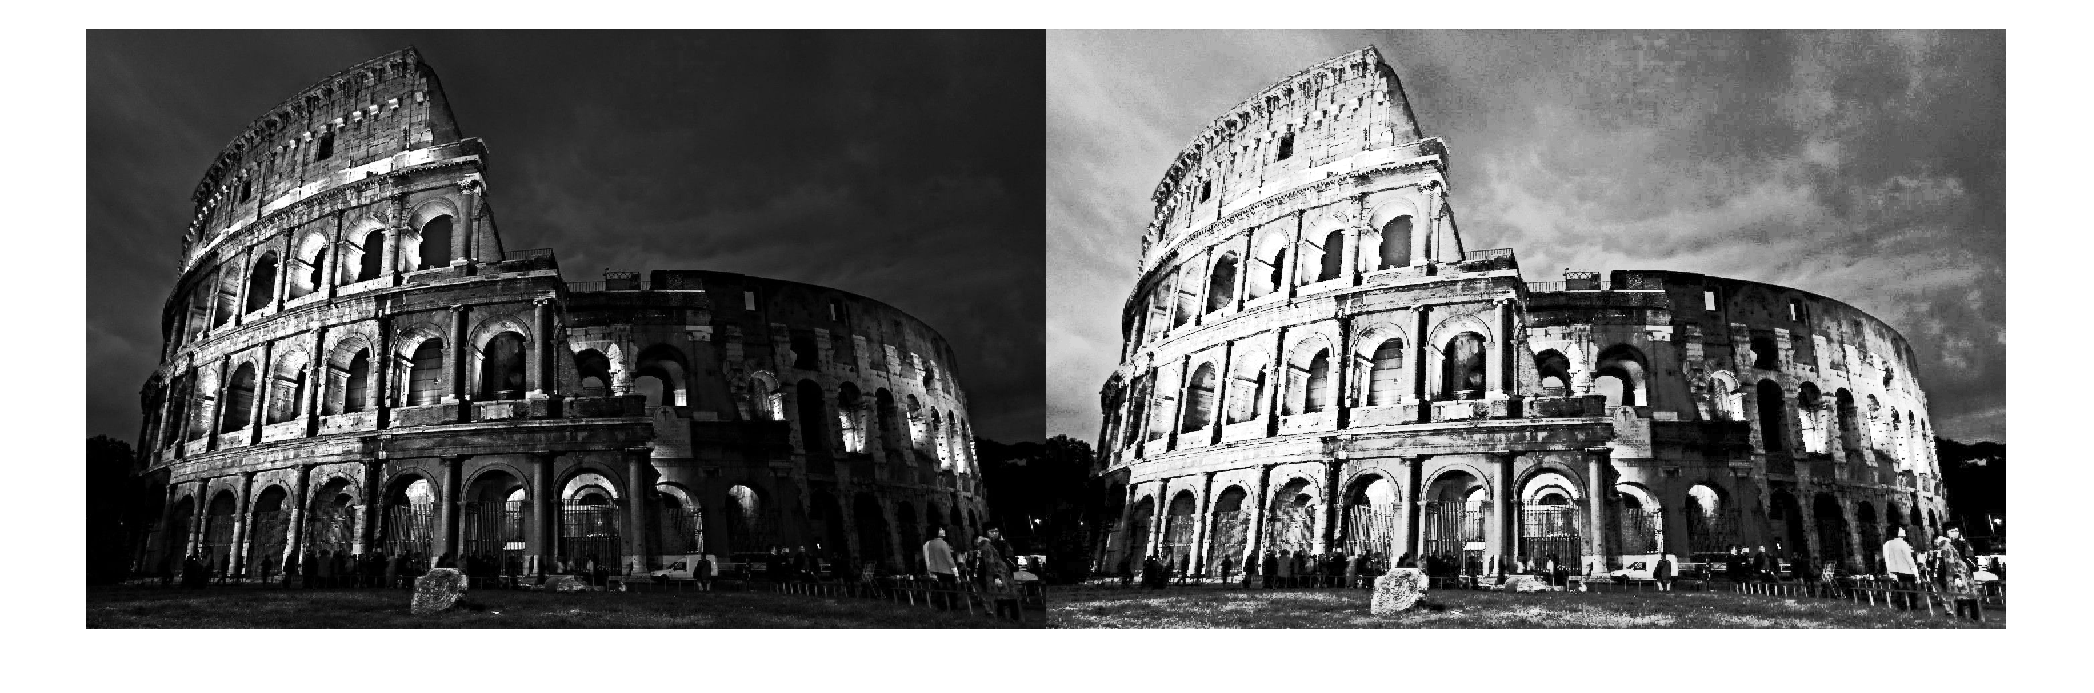
\includegraphics[width=0.75\textwidth]{../figures/eq1}
		\caption{直方图均衡化}
		\label{1}
	\end{figure}
	\begin{figure}[h!]
		\centering
		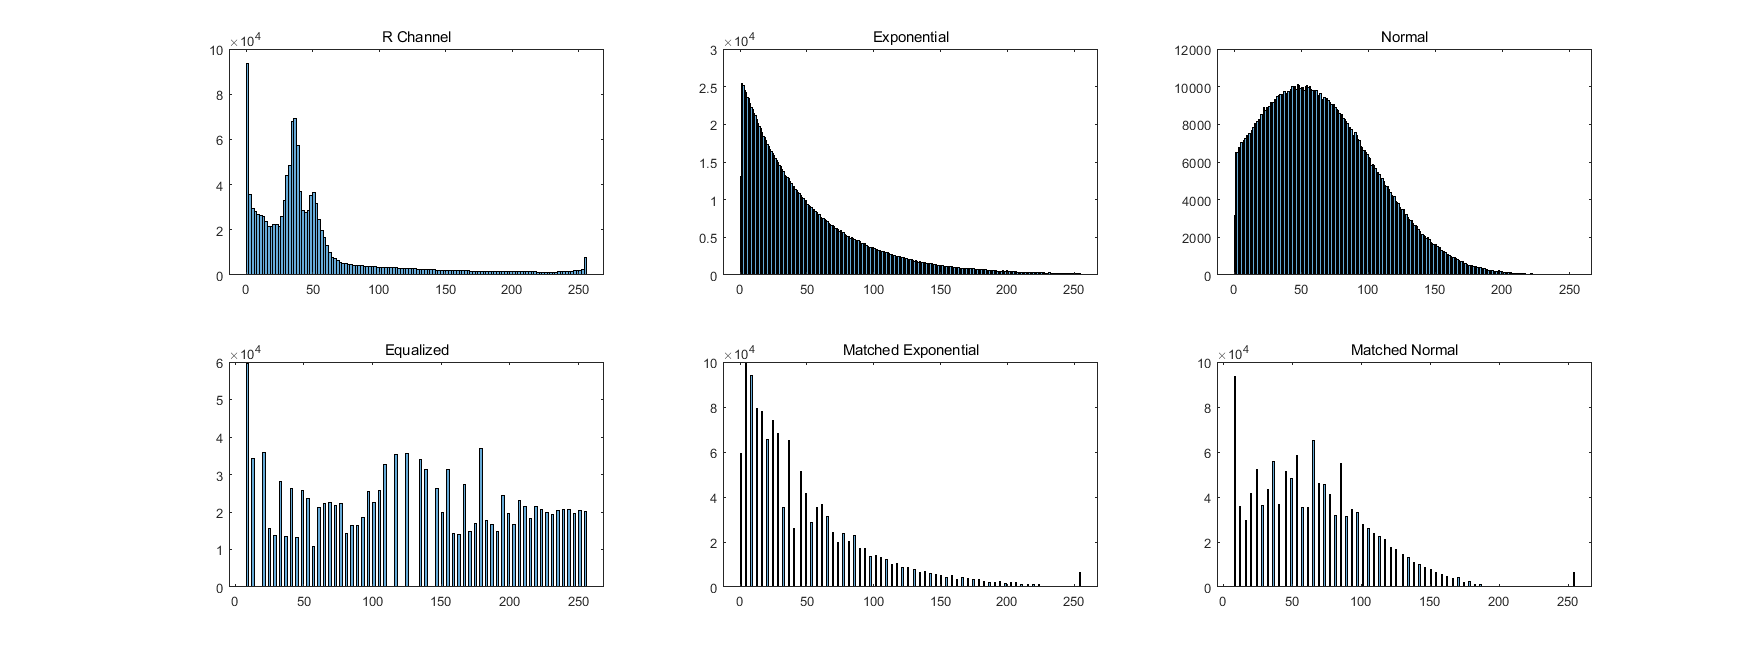
\includegraphics[width=1\textwidth]{../figures/hists1}
		\caption{（1）（2）部分直方图}
		\label{2}
	\end{figure}
	\begin{figure}[h!]
		\centering
		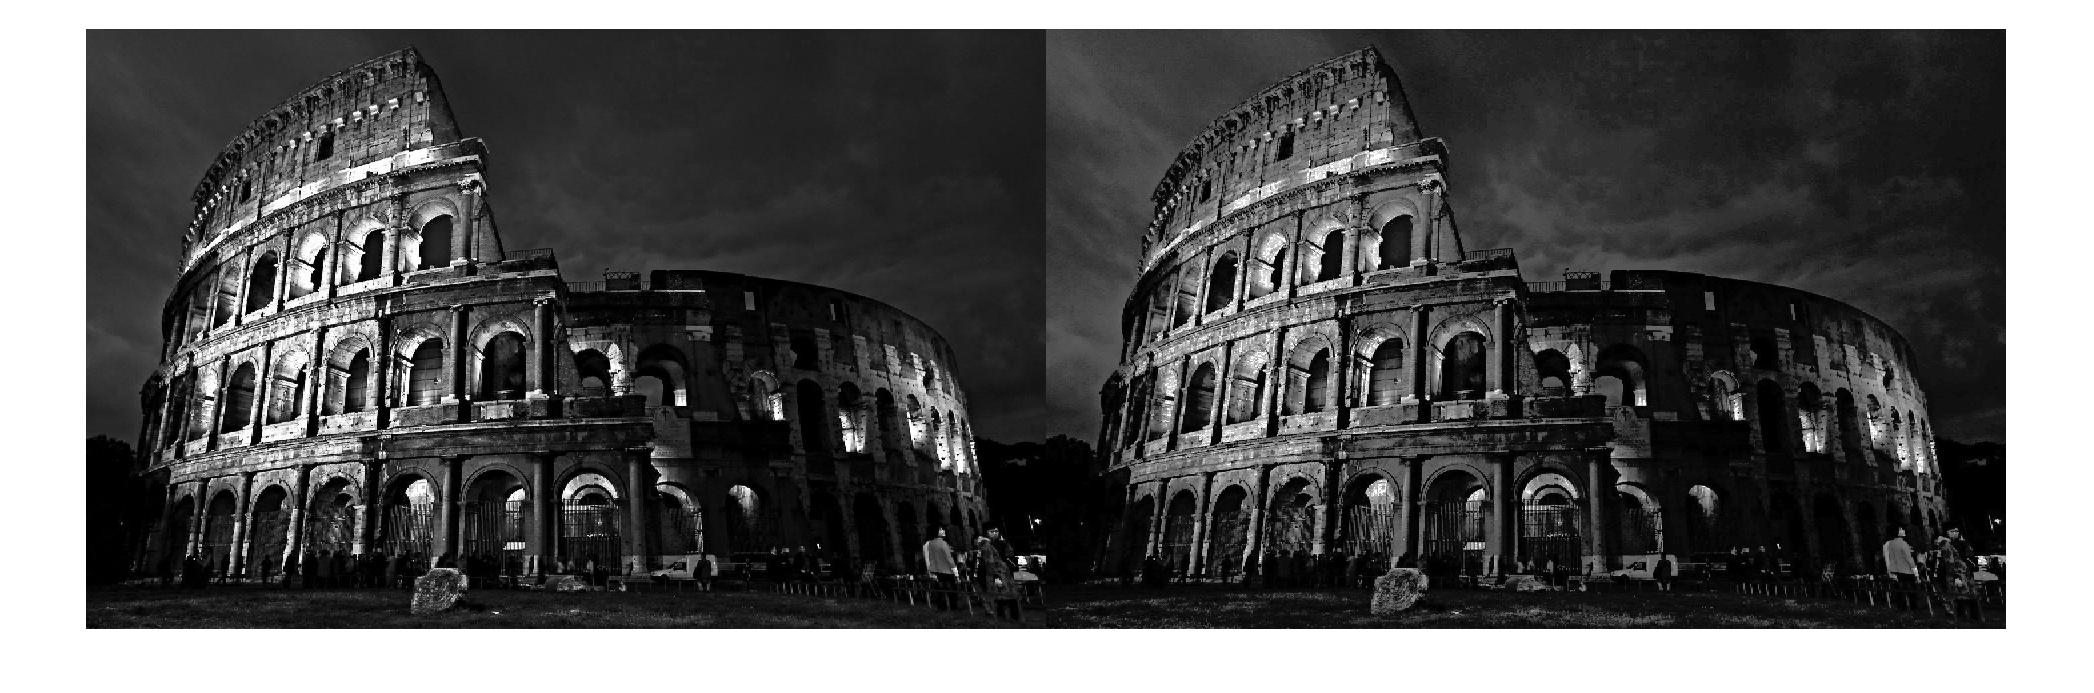
\includegraphics[width=0.75\textwidth]{../figures/exp1}
		\caption{指数匹配}
		\label{3}
	\end{figure}
	\begin{figure}[h!]
		\centering
		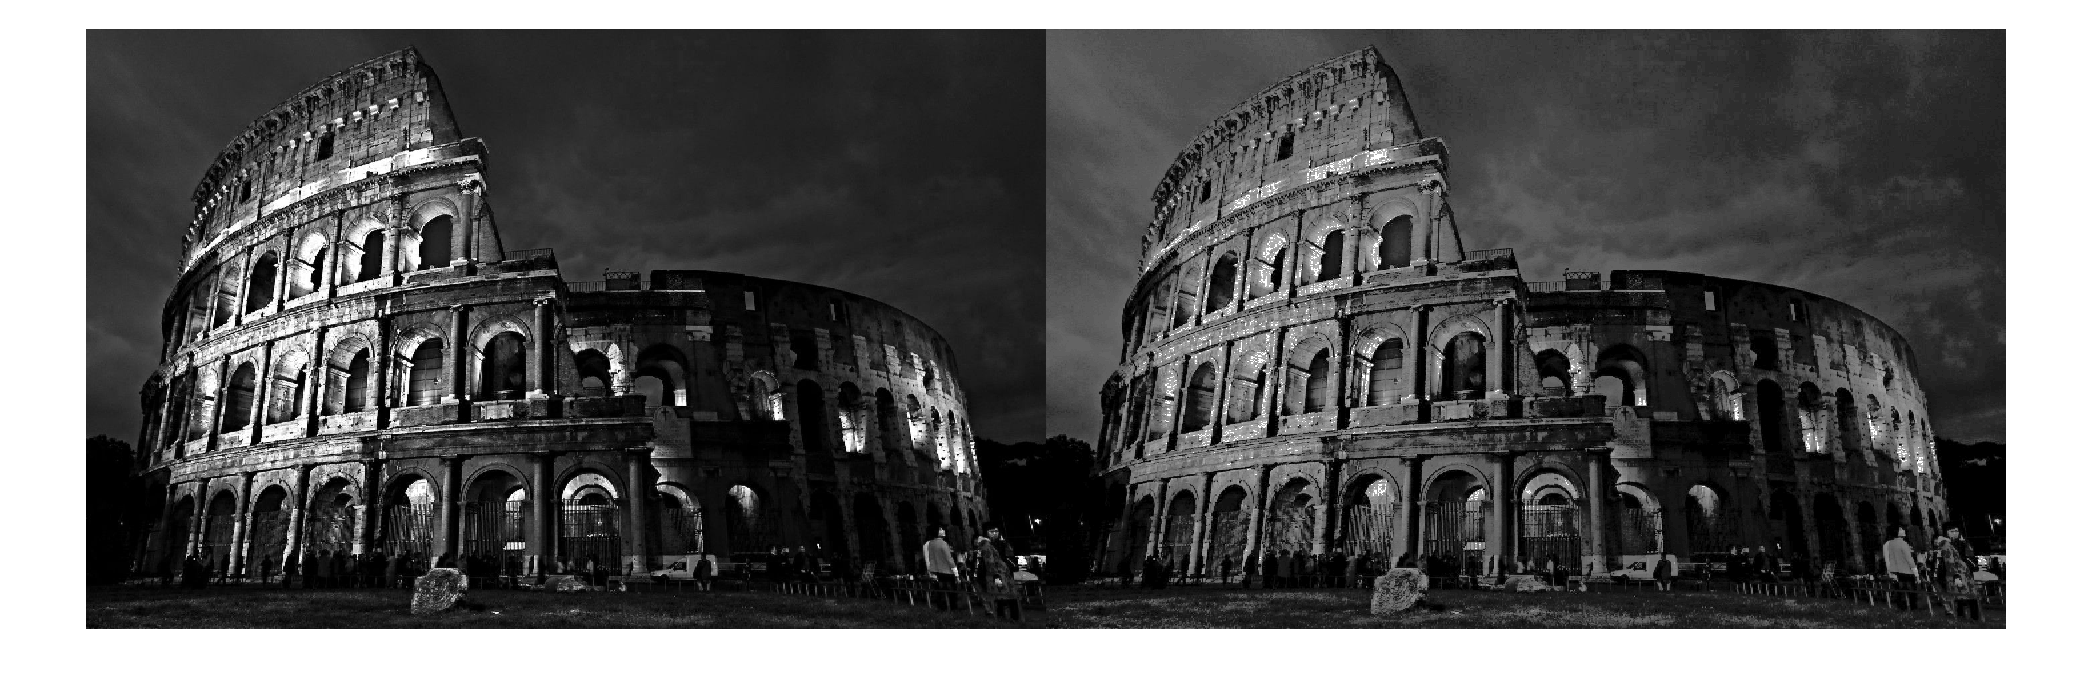
\includegraphics[width=0.75\textwidth]{../figures/norm1}
		\caption{高斯匹配}
		\label{4}
	\end{figure}
	\begin{figure}[h!]
		\centering
		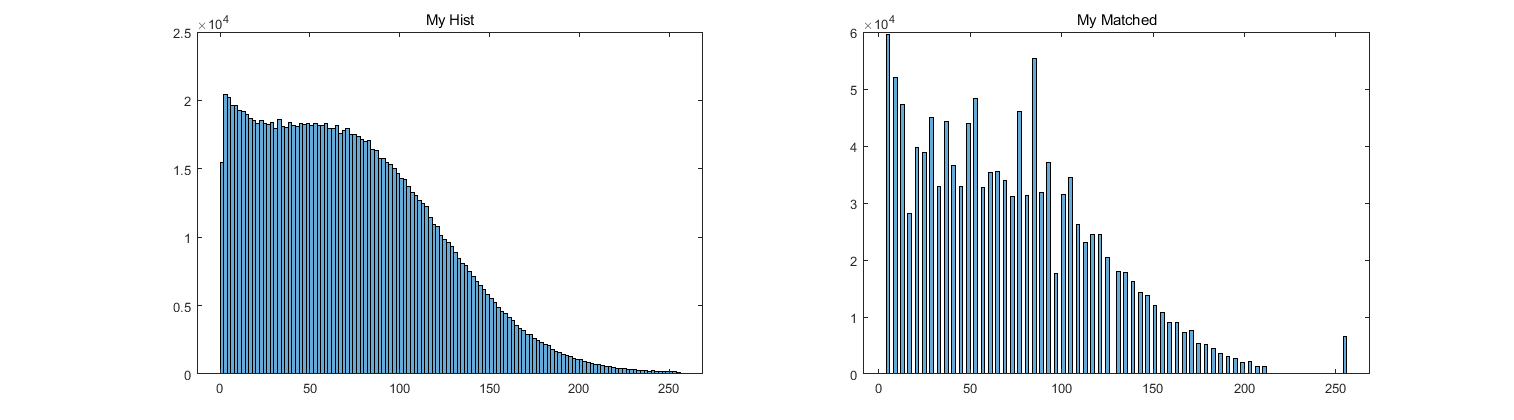
\includegraphics[width=1\textwidth]{../figures/myhist}
		\caption{设计直方图}
		\label{5}
	\end{figure}
	\begin{figure}[h!]
		\centering
		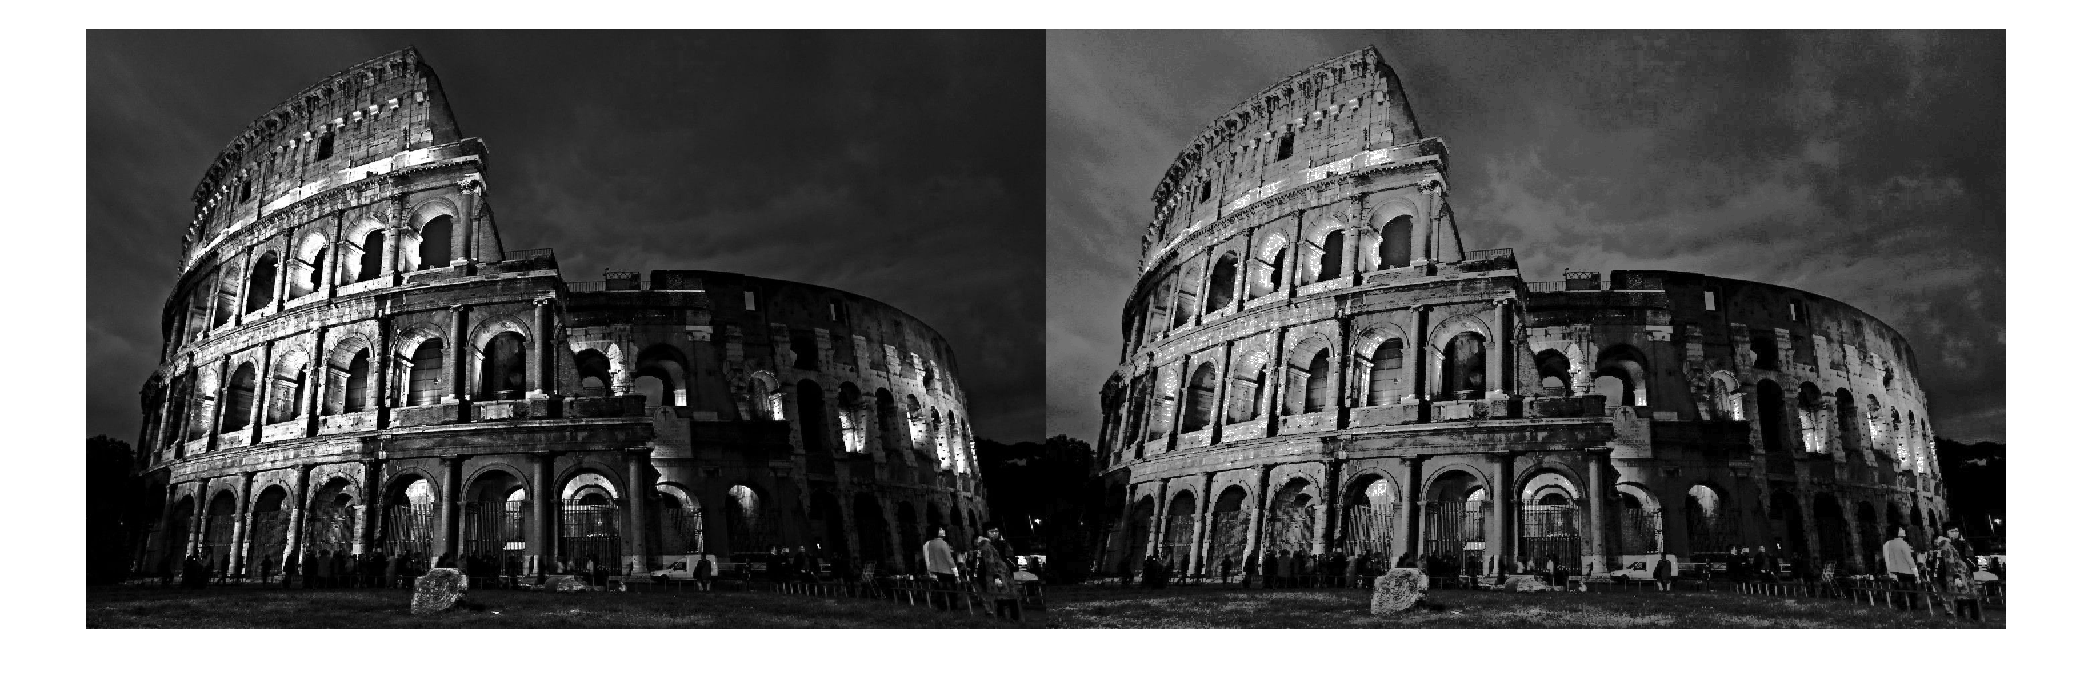
\includegraphics[width=0.75\textwidth]{../figures/myresult}
		\caption{设计效果}
		\label{6}
	\end{figure}
	\begin{figure}[h!]
		\centering
		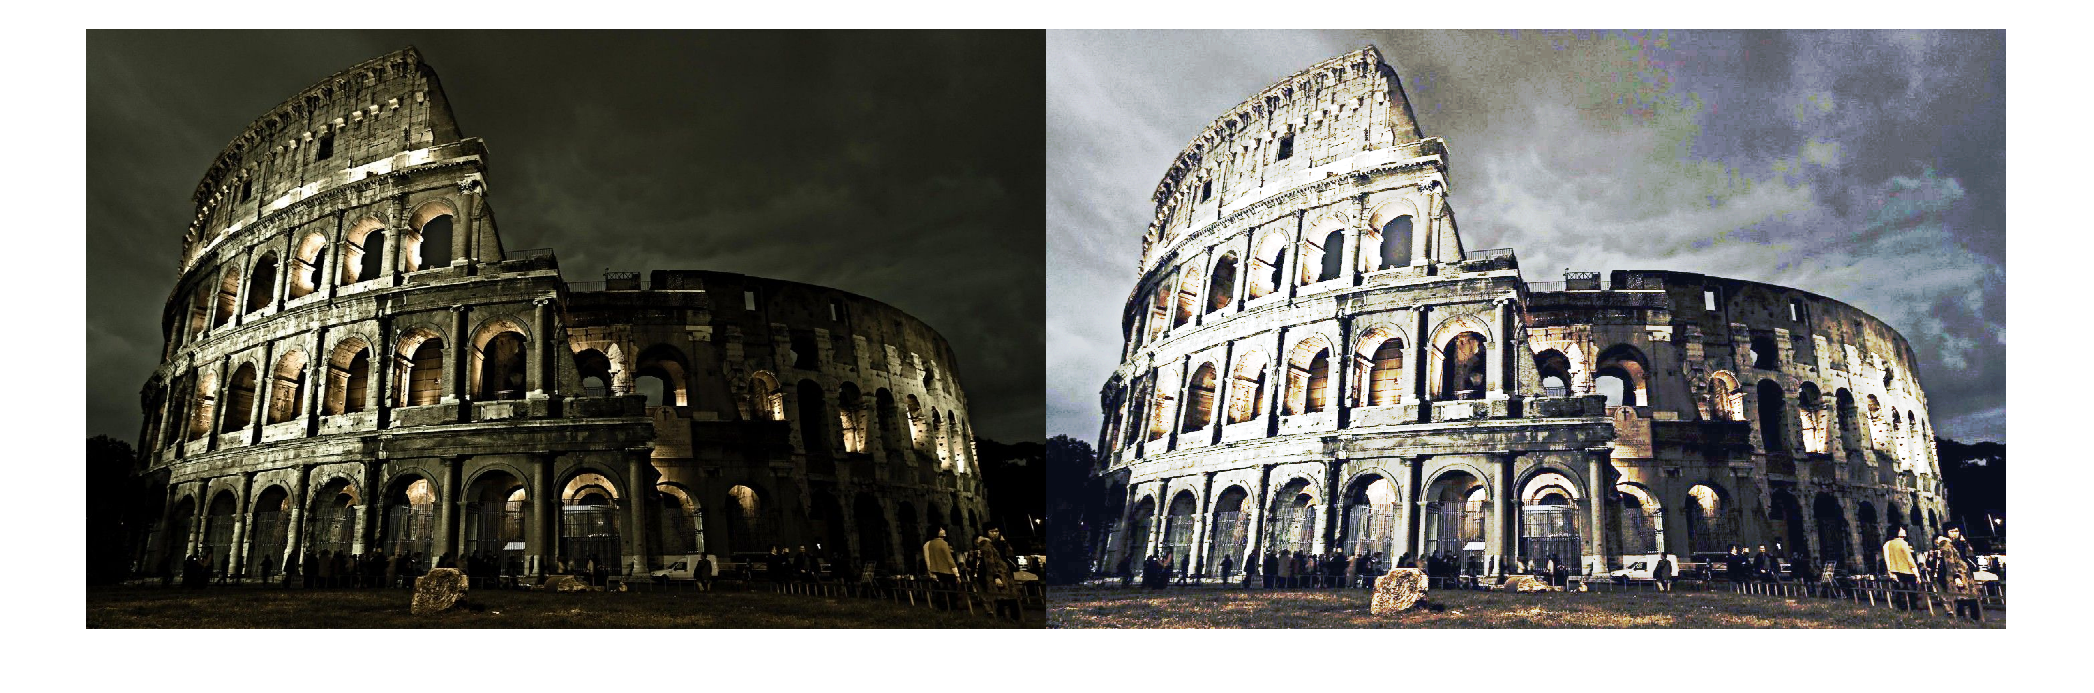
\includegraphics[width=0.75\textwidth]{../figures/rgbequ}
		\caption{RGB均衡化}
		\label{7}
	\end{figure}
	\begin{figure}[h!]
		\centering
		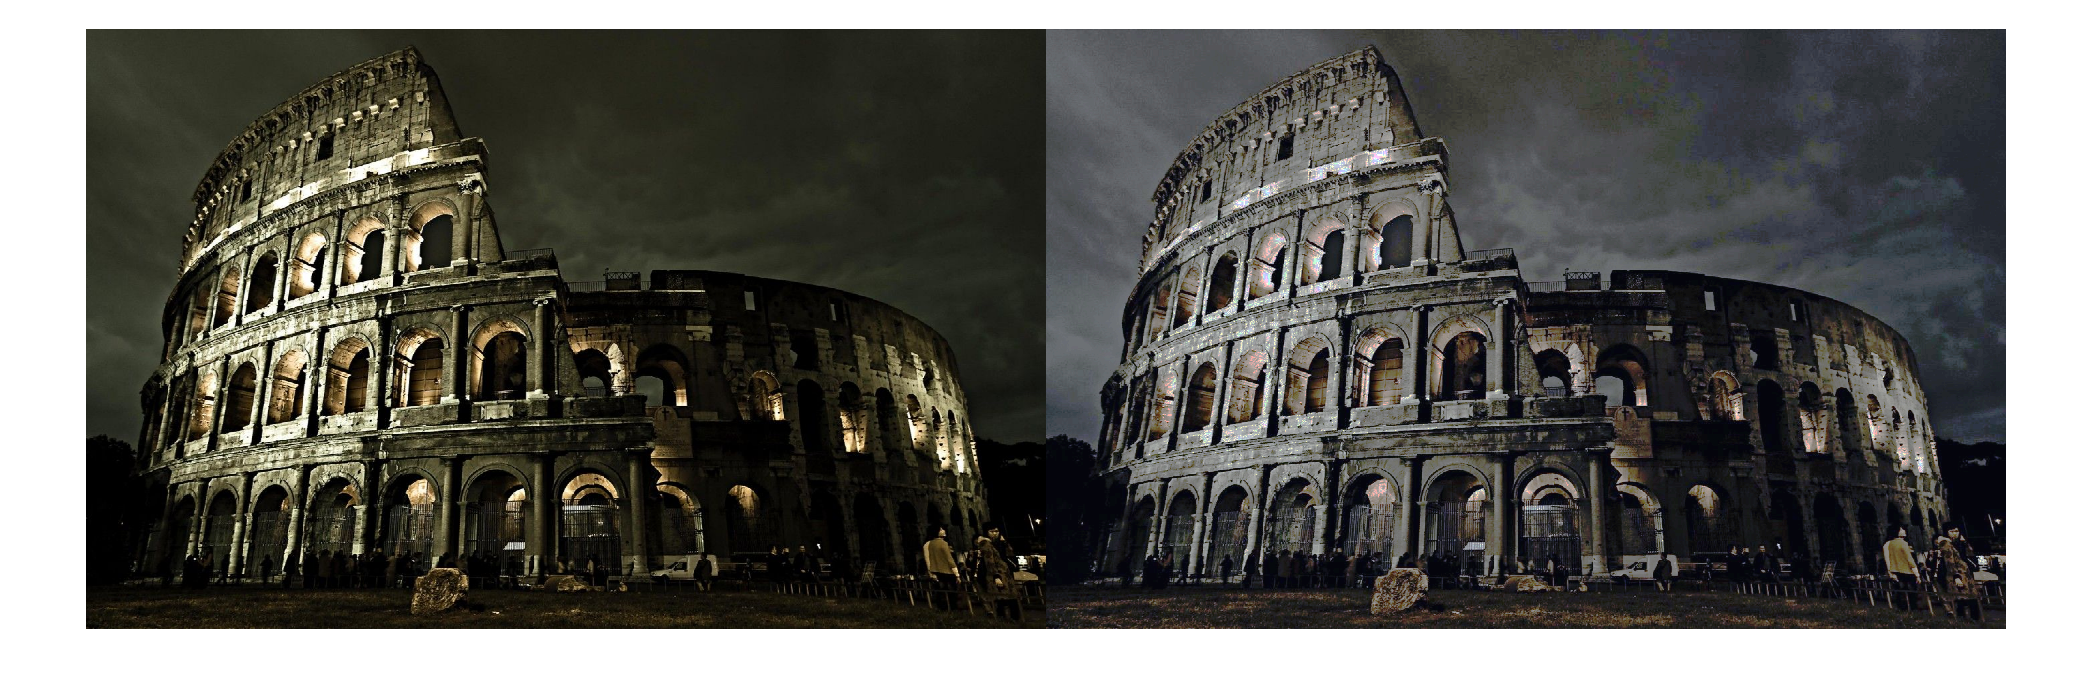
\includegraphics[width=0.75\textwidth]{../figures/myres}
		\caption{最终结果}
		\label{8}
	\end{figure}
\end{document}